\documentclass[a4paper,12pt]{article}

\usepackage{fancyhdr}
\lhead{\footnotesize{Project CUDC Proposal}}
\lfoot{\footnotesize{CS 217 Fall 2015}}
\rfoot{\footnotesize{OUNAN DING 861194909}}
\pagestyle{fancy}

\usepackage{hyperref}

\usepackage{amsmath}

% For \mathds
\usepackage{dsfont}

\usepackage{graphicx}

\title{Project CUDC Proposal}
\date{}
\author{
OUNAN DING\\
Student ID: 861194909\\
oding001@ucr.edu
}

\begin{document}

\maketitle{}

\tableofcontents{}

\section{Abstract}

In this document we propose a
\underline{CU}DA based \underline{D}ual \underline{C}ontouring(CUDC)
project.
The computation model of dual contouring will be studied,
then the data and computation parallelism will be exploited
for a CUDA based implementation.
A CPU based reference implementation will be provided as well.
The profiling and benchmarking will be taken on these two implementations.
Finally a conclusion
will be reached based on our implementation, profiling, and analysis.

\section{Technique Overview}
Dual contouring is a technique that converts
a implicit function \cite{ wiki:implicit-function}
to mesh,
which is a collection of vertices, edges, faces \cite{wiki:polygon-mesh}.
The general theoretical foundation of this project
is outlined by \cite{ju2002dual}. We will give an overview of it here.

Given an implicit function like $x^2 + y^2 + z^2 = c$,
we can use dual contouring to construct the surface mesh
at the level set $c$, that is, the surface of a 3D sphere.

Concretely, in dual contouring,
a function $f(x) = x^2 + y^2 + z^2$ is evaluated at discrete grid vertices
in a portion of space.
And for each vertex at $(x_i, y_i, z_i)$, we can determine if it belongs to
the interior or the exterior of geometry
based on the sign of $f(x_i, y_i, z_i)$.
After that we can use this information to construct mesh for the geometry.

In some previous research, such as marching cube \cite{lorensen1987marching},
the sharp features are not preserved in constructed mesh.
Whereas in dual contouring, we extract the Hermite data
from the original implicit representation,
and construct Quadratic Error Functions(QEF)
as a more accurate model of features in original geometry.

By solving the QEFs in the grid we can get the mesh vertices.
Finally we connect the adjacent vertices to build the topology of mesh.

I have already had a working example of 3D dual contouring in Python
\cite{learnblenderdev-3d-dc}.
The running result is shown in \ref{fig:3d-dc-python}, where a 3D heart function
$(2 x^2 + y^2 + z^2 - 1)^3 - x^2 z^3 / 10 - y^2 z^3 = 0$
is contoured.

By using CUDA, we expect a performance boost in this application.

\begin{figure}[h]
\centering
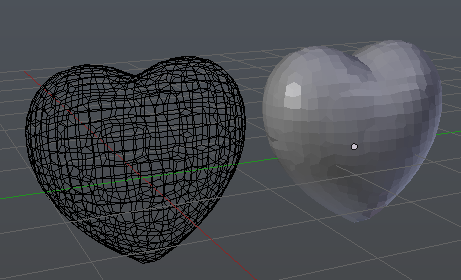
\includegraphics{heart-function-3d-dc.png}
\caption{A working example of 3D dual contouring from \cite{learnblenderdev-3d-dc}}
\label{fig:3d-dc-python}
\end{figure}

\section{Requirements}

\subsection{User Inputs}

Users are expected to input a string of function definition
($\mathds{R}^3 \rightarrow \mathds{R}$ in 3D case,
or $\mathds{R}^2 \rightarrow \mathds{R}$ in 2D case) to our application.
Then our application will parse users' input and generate a kernel function
at the runtime.

However, the generating of kernel function at runtime
requires NVRTC, which is introduced with NVIDIA CUDA toolkit version 7.0.
In our storm server the version of installed CUDA toolkit is 5.0.
We work around this by hard coding the function definition
in the source code.

\subsection{Host-Device Data Transfer}

Every cell in the computation grid may output a generated mesh vertex.
We need to allocate the memory for them.
Since only surface of the geometry will be contoured,
we expect a space complexity of $\mathcal{O}(n^2)$
($n$ is the dimension of one side of the computation grid) in 3D case,
or $\mathcal{O}(n)$ in 2D case.

\subsection{Function Evaluation}

Since the computation of input function at grid vertices
is completely independent,
we can utilize the CUDA for optimal performance.
This should easily outperform a CPU implementation.

\subsection{Intersection Detection}

We need to check the $8$ vertices(or $4$ vertices in 2D case)
to determine if an edge intersects with the geometry surface.
This requires irregular memory access on the grid.
It will be a challenge to achieve the maximal performance.

Besides, only a portion of the cells in the grid may intersect with
the geometry. Hence a stream compaction is required here.

\subsection{Hermite Data Generation}

In this stage we need to compute the
exact intersection point and the surface normal(i.e. the Hermite data)
for each edge which exhibits an intersection.

The surface normal is computed
by a finite differencing over the implicit function.
And it can be fully parallelized due to the independence in computation.

However the exact interaction position is computed by a bisect search.
This may cause branch(divergence).

\subsection{Quadratic Error Function}

To solve a QEF we need to perform a pseudo-inverse.
Usually this is done through SVD or QR decomposition.
We want a coherent algorithm here.
This is the place where the majority work goes.

\subsection{Mesh Topology Construction}

The mesh topology construction usually is not a bottleneck.
And this work does not fit the SIMT programming model very well.
So I am thinking to implement it in host/CPU side in our first try.

However, for some applications such as real time rendering,
the generated mesh data will be sent to the GPU rasterization pipeline
for rendering.
Thus the overhead of
an extra data transfer from GPU to CPU
cannot be ignored.
We will optimize this in later phase of this project.

\subsection{Visualization}

After we fetch the result data from device,
we need a program to visualize it for correctness.
This can be done by using a 3D modeling software or an ad-hoc renderer using
graphics API such as Direct3D or OpenGL.

\subsection{The Baseline and Profiling}

We also provide a CPU implementation as our reference and baseline
during the benchmark.
The CUDA implementation will be profiled and analyzed
to reach our final conclusion.

\section{Outputs}

A CPU implementation will be provided as reference and baseline;
a CUDA implementation will be provided, optimized, profiled, and analyzed;
a report on the project process and performance analysis will be written.

\newpage
\addcontentsline{toc}{section}{References}
\bibliography{papers,wikipages,others}
\bibliographystyle{alpha}

\end{document}
